\documentclass{IEEEtran}

%\author{Piers R. Williams, \and Joseph Walton-Rivers}

\title{MCTS Applied to Co-operative Problems}

\usepackage{graphicx}
\usepackage{glossaries}

\graphicspath{{stats-processing/}{stats-processing/data/maps/}}

\newacronym{mcts}{MCTS}{Monte-Carlo Tree Search}
\newacronym{uct}{UCT}{Upper Confidence bound applied to Trees}
\newacronym{ggp}{GGP}{General Game Playing}
\newacronym{ga}{GA}{Genetic Algorithm}
\newacronym{mas}{MAS}{Multi-Agent Systems}
\newacronym{maga}{MAGA}{Macro Action Genetic Algorithm}
\newacronym{ai}{AI}{Artificial Intelligence}

\begin{document}
\maketitle
\begin{abstract}
This paper highlights an experiment to see how standard MCTS handles simple co-operative problems with no prior or provided knowledge. These problems are formed from a simple grid world that has a set of goals, doors and buttons as well as walls that cannot be walked through. Two agents have to each reach every goal present on the map. For a door to be open, an Agent must be present on at least one of the buttons that is linked to it.

When laid out correctly, the world requires each agent to do certain things at certain times in order to achieve the goal. With no modification to allow communication between the two Agents - MCTS performs well and performs very 'purposefully' when given enough computational time.
\end{abstract}

\section{Introduction}
\gls{ggp} is the field of writing \gls{ai} agents that can play a multitude of games without being written specifically for each one individually. \gls{ggp} in real time video games is a popular competition \cite{perez2014}

Creating \gls{ggp} agents that can co-operate with other players would open the door for more flexible agents in games that can work together with human players. This experiment tests how well current techniques can cope without specifically co-operating with each other. Agents that communicate slowly using a form of Natural Language, should in theory be able to work with human players equally well as they do with other Agents.

\gls{mcts} \cite{browne2012survey} has been applied to a wealth of domains and is one of the primary algorithms in use for \gls{ggp}\cite{finnsson2008simulation}. Primary advantages are that, when given a sufficient forward model, \gls{mcts} doesn't require any knowledge about the game itself in order to play.

Standard \gls{mcts} plays best when it is either able to search to the end of the game tree, or is given rewards frequently. \gls{mcts} tends to stumble when the time given to it isn't sufficient to allow it to locate any sequence of actions that provides a reward in order to differentiate the root's children \cite{perez2012monte}.

\section{The Experiment}
The main premise was to put \gls{mcts} in a situation where it would rely on other AI Agents in order to achieve its objectives, as well as provide a code base for further work with communication between Agents. In order to do this, a problem domain was created.
\subsection{The Problem Domain}
The problem domain is a simple grid world consisting of various objects:
\begin{itemize}
\item{\emph{Floor - } Floors are passable, and are rendered in Grey.}
\item{\emph{Walls -} Walls are impassable, and are fixed in position. \emph{Walls} are rendered in Black.}
\item{\emph{Agents -} Agents are the moving objects that can activate buttons and the goal. \emph{Agents} are rendered in dark Yellow}
\item{\emph{Doors -} Doors can either be open or closed. When open, the door is passable. When closed, the door is impassable. Doors are open whilst an \emph{Agent} is activating a linked \emph{Button}. If the \emph{Agent} stops activating the \emph{Button} the \emph{Door} will close. \emph{Doors} are rendered in Blue when closed, and are invisible when open.}
\item{\emph{Buttons -} Buttons are passable, and when an \emph{Agent} is on the \emph{Button} it will activate and open the linked \emph{Door}. \emph{Buttons} are rendered in Red}
\item{\emph{Goals -} Goals are passable and reward all \emph{Agents} with a portion of the score. All \emph{Goals} are worth the same amount and the maximum score of $1$ is achieved when every \emph{Agent} has visited every \emph{Goal} at least once. Re-visiting a \emph{Goal} has no effect. \emph{Goals} are rendered in Bright Yellow}
\end{itemize}

The starting positions for a simple problem is shown in Figure \ref{InitialState}
\begin{figure}[ht]
\centering
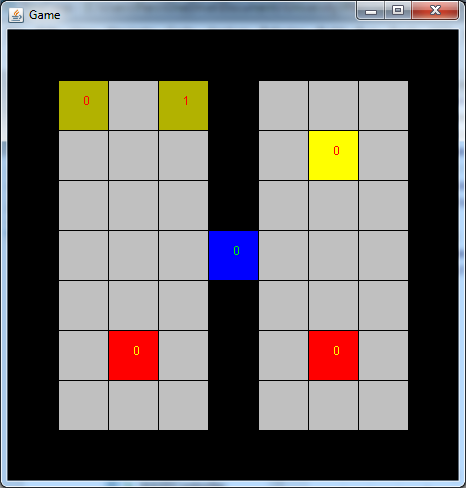
\includegraphics[scale=0.5]{InitialState}
\caption{Simple game state showing the different elements\protect\footnotemark }
\label{InitialState}
\end{figure}

\footnotetext{Displayed numbers are the ID numbers - \emph{Button} ID 0 will open \emph{Door} ID 0 but not \emph{Door} ID 1}
All levels are defined by a simple text file format.

The problems are designed to require \emph{Agents} to co-operate in order to achieve their goals. Unlike other environments where \gls{mcts} can charge off achieving its own goals, this domain requires the agents to sometimes sit patiently on a button for another Agent to do something else.

\subsection{Initial Testing}
Initially, observations were made to see how \gls{mcts} handled the problem. At first, with a small computational budget it seemed like \gls{mcts} would perform poorly, with near random movement seeming to emerge.

This changed, when an agent (Agent 1 say) got near a \emph{Button} or \emph{Door}. When Agent 1 reached an item like this - Agent 2 would seemingly gain some purpose and typically head for the other items. When Agent 1 got on the \emph{Button}, Agent 2 would head straight through the open \emph{Door} and to the \emph{Goal}. Behaviour would then typically go back towards a more random approach, unless the Agent 1 got near the \emph{Door} - typically causing Agent 2 to head more purposefully towards the \emph{Button} that would allow Agent 1 to reach the \emph{Goal}.

With this observation made - the computational budget was increased ten-fold, and the \gls{mcts} agents performed significantly better. Typical behaviour would be near optimal with significantly less random sections of movement. This can likely be attributed to the increased rollout and \gls{uct} border depths allowing more foresight on such a small puzzle.
\subsection{Tournament}
For the main data collection, we ran a round robin tournament of maps and Agents.

\subsubsection{Maps}
The 7 maps that were included in the tournament were as follows:
\begin{itemize}
\item{\emph{level1.txt} This map is the same as the map in \ref{InitialState}}
\item{\emph{level1E.txt} This map is the same as level1.txt but without the \emph{Doors} and \emph{Buttons}. This was to test the \emph{Agent's} ability to solve the simplest problem.}
\item{\emph{level2.txt} This map was a modification of the level1.txt - making the map more symmetric and the action parts closer together.}
\item{\emph{level3.txt} This map was an extension of level1.txt with a second \emph{Goal} and some extra walls in the game. Spreading the action parts away from the door and buttons was the main purpose of this one}
\item{\emph{level4.txt} This map was a modification of level1.txt - putting a second \emph{Goal} in and making the map partly mirrored. Each \emph{Agent} began in a separate room to each other instead of together.}
\item{\emph{level5.txt} This map was a new map, designed to give wildly different roles to each AI - the top Agent would have to travel through two doors that the bottom agent had access to the linked \emph{Buttons}. Then the top \emph{Agent} could collect the reward and allow the bottom \emph{Agent} access to the \emph{Goal}.}
\item{\emph{level6.txt} This map was a new map - with two rooms each with a \emph{Goal} and a door.This was designed to force each \emph{Agent} to be let into the \emph{Goal} room, and out of it again.}
\end{itemize}

\subsubsection{\gls{ai} Controllers}
A small set of \gls{ai} Controllers were created in order to attempt to solve the problem domain. None of the agents have the ability to communicate with another agent.
\paragraph{Random}
The random controller simply chooses one of the possible 5 actions. This is one of the simplest to implement and run.
\paragraph{Keyboard}
The keyboard controller takes input from the keyboard and translates that into a single Action. Once an action is polled, it is reset to the No Op action unless the keyboard is used again. 
\paragraph{\gls{mcts}}
The \gls{mcts} controller is a simple implementation of \gls{uct} - with a fixed iteration, \gls{uct} Border and rollout border. No knowledge about the game is provided and the assumption is made that the other player will play randomly. The fixed rollout border makes a significant improvement in iterations per decision (from 1-3 to 500-600 in 40ms \footnote{Intel Core i5-3570, 8GB RAM, Windows 7 Enterprise 64bit}). This greatly improves the ability of \gls{mcts} to make informed decisions. The score at the end of a rollout is taken from the game state - so if \gls{mcts} doesn't see any player reach a goal, all branches will be equal.

For the tournament, three parameter sets were chosen for comparison and are shown in Figure \ref{mctsTable}.
\begin{figure}[h]
\centering
\begin{tabular}{| l | c | c | c |}
\hline
\textbf{Budget} & \textbf{Iterations} & \textbf{Max UCT} & \textbf{Max Rollout} \\
\hline
Small & 75 & 3 & 15 \\
Medium & 200 & 5 & 30 \\
High & 500 & 10 & 45 \\
\hline
\end{tabular}
\caption{Table of parameters for the 3 \gls{mcts} players}
\label{mctsTable}
\end{figure}

\paragraph{Macro Action Genetic Algorithm}
The \gls{ga} algorithm was selected for its simplicity and had Macro Actions added in order to improve the forward search capability. The \gls{maga} used a population size of 10 and tournament selection of 3. Each candidate was a string of 15 actions - with each action performed 3 times in a row. This meant the \gls{maga} could "see" 45 ticks in the future.
\paragraph{Variable Macro Action Genetic Algorithm}
The Variable Macro Action \gls{ga} was created to try to solve the shortcomings of \gls{maga}. The primary premise was to allow the \gls{ga} to evolve the individual macro action lengths and the length of the overall sequence (number of macro actions). The main technique used was a 1 + 1 ES. The algorithm was bounded by a number of parameters that are shown in Figure \ref{vmagaTable}.

\begin{figure}[h]
\centering
\begin{tabular}{| l | l | l |}
\hline
\textbf{Param} & \textbf{Controls} & \textbf{Value} \\
\hline
minNum & Number of Macro Actions & 3 \\
MaxNum & Number of Macro Actions & 10 \\
minLength & Length of Macro Actions & 1 \\
maxLength & Length of Macro Actions & 5 \\
numChance & Chance of altering Number & 0.25 \\
lengthChance & Chance of altering each length & 0.8 \\
actionChance & Chance of altering each action & 0.75 \\
\hline
\end{tabular}
\caption{Table of parameters for the Variable Macro Action Genetic Algorithm}
\label{vmagaTable}
\end{figure}
These values need extensive tuning to realise the full potential of the algorithm and is a source of possible future work.
\pagebreak
\section{Results}

\begin{figure}[ht]
\centering
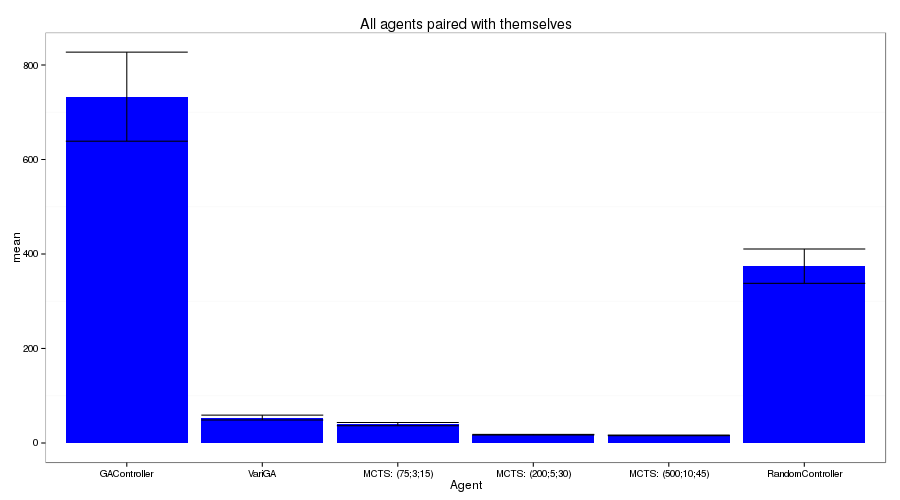
\includegraphics[width=\linewidth]{level1E-txt-pairs-ticks}
\caption{Average ticks taken to complete level1E.txt when paired only with identical Agents}
\label{1epairedTicks}
\end{figure}

\begin{figure}[ht]
\centering
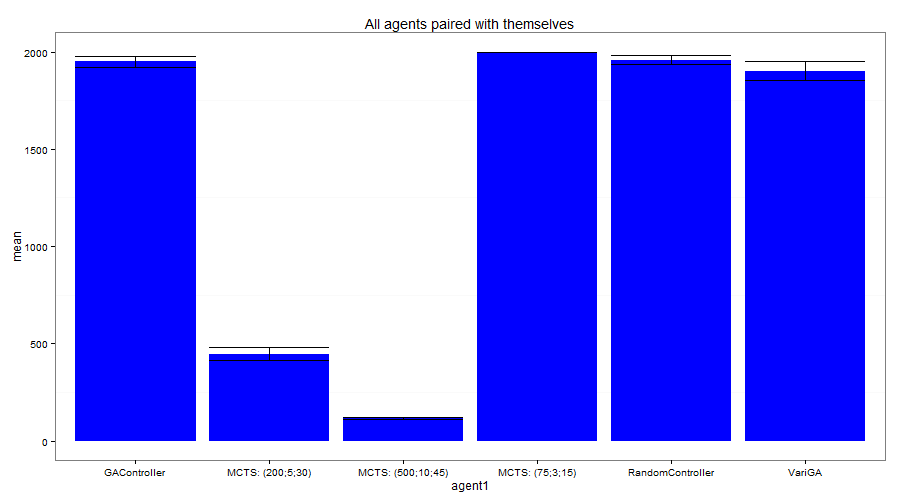
\includegraphics[width=\linewidth]{level1-txt-pairs-ticks}
\caption{Average ticks taken to complete level1.txt when paired only with identical Agents}
\label{1pairedTicks}
\end{figure}

Figure \ref{1epairedTicks} shows the ability of each Agent to solve a simple path finding problem. The \emph{GAcontroller}, with its macro actions, is hindered by its inability to make single step moves and has trouble actually walking straight to the target. The \emph{VariGA} does significantly better, due to its ability to perform single step moves. Figure \ref{1pairedTicks} shows that most of the controllers really struggle when the \emph{Door} and \emph{Buttons} are added. This proves that the challenge of the task is high, although perhaps remarkable that \gls{mcts} is able to solve the tasks.

\begin{figure}[ht]
\centering
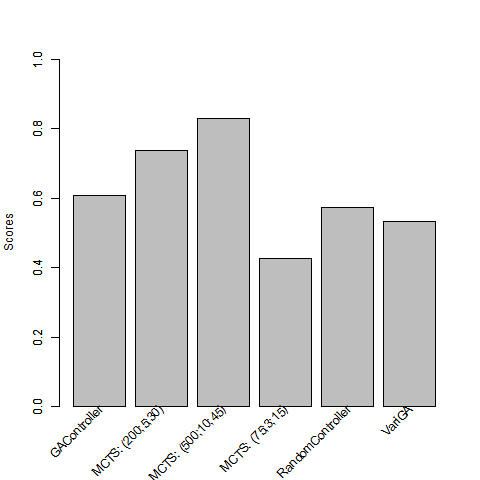
\includegraphics[width=\linewidth]{scores-allmaps}
\caption{Average score of each AI Agent over all the Maps}
\label{avgScoreAllMaps}
\end{figure}

\begin{figure}[ht]
\centering
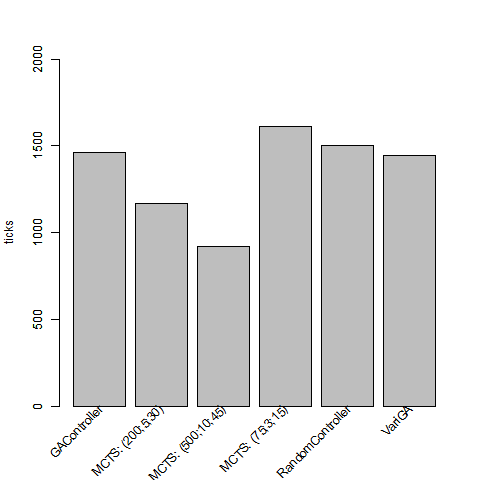
\includegraphics[width=\linewidth]{ticks-allmaps}
\caption{Average Ticks taken for each AI Agent over all the Maps}
\label{avgTicksAllMaps}
\end{figure}

\begin{figure}[ht]
\centering
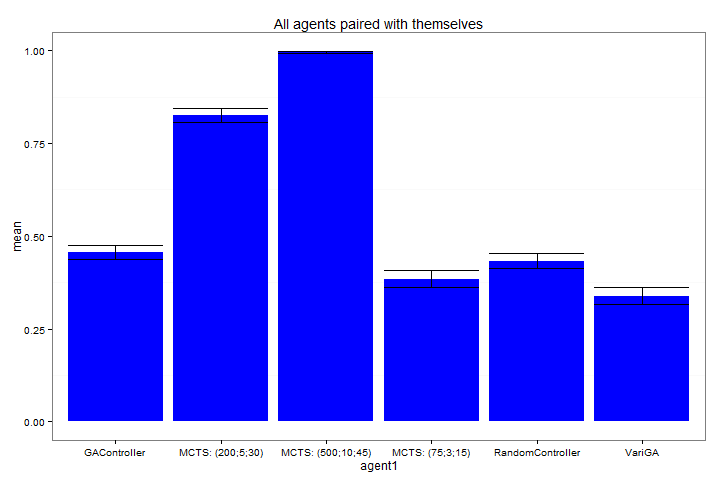
\includegraphics[width=\linewidth]{scores-samepairs}
\caption{Average Scores for each AI Agent paired with itself over all the Maps}
\label{avgScorePairAllMaps}
\end{figure}

\begin{figure}[ht]
\centering
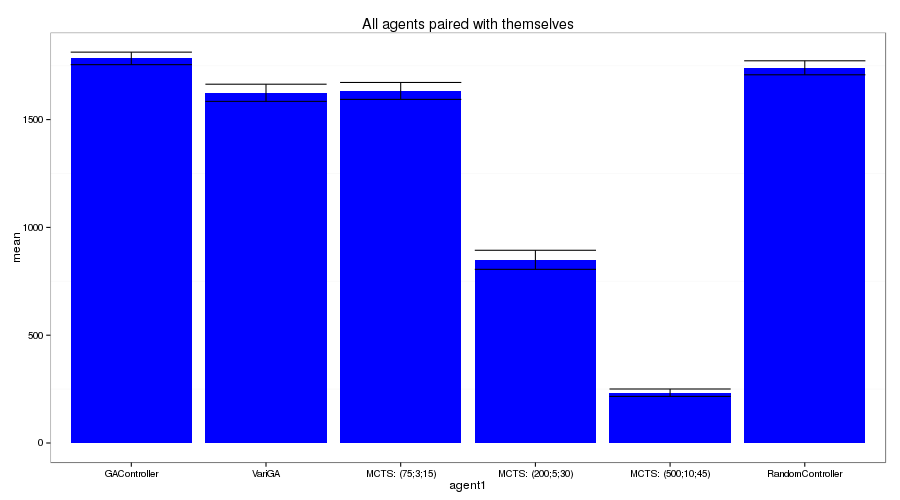
\includegraphics[width=\linewidth]{ticks-samepairs}
\caption{Average Ticks taken for each AI Agent paired with itself over all the Maps}
\label{avgTicksPairAllMaps}
\end{figure}

Figure \ref{avgScoreAllMaps} shows the average score that each AI Agent achieved over all the maps. The two more powerful \gls{mcts} Agents performed the best, doing much better than the competition. Figure \ref{avgTicksAllMaps} shows a similar result, with the more powerful Agents typically completing the maps in fewer ticks. \emph{RandomController} is the only deviant here - it outperformed the GA's in score but was worse in average ticks. Comparing the \gls{ai} \emph{Agents} when paired only with themselves in Figure \ref{avgScorePairAllMaps} and Figure \ref{avgTicksPairAllMaps}. The shockingly good results for \emph{RandomController} are potentially due to the fact that the 3 \gls{mcts} controllers and 2 \gls{ga} algorithms all based their decisions on having Random as an accomplice.

\pagebreak
\begin{figure}[ht]
\centering
\includegraphics[scale=0.5]{level5}
\caption{The initial starting state for level5.txt}
\label{Level5State}
\end{figure}

\begin{figure}[ht]
\centering
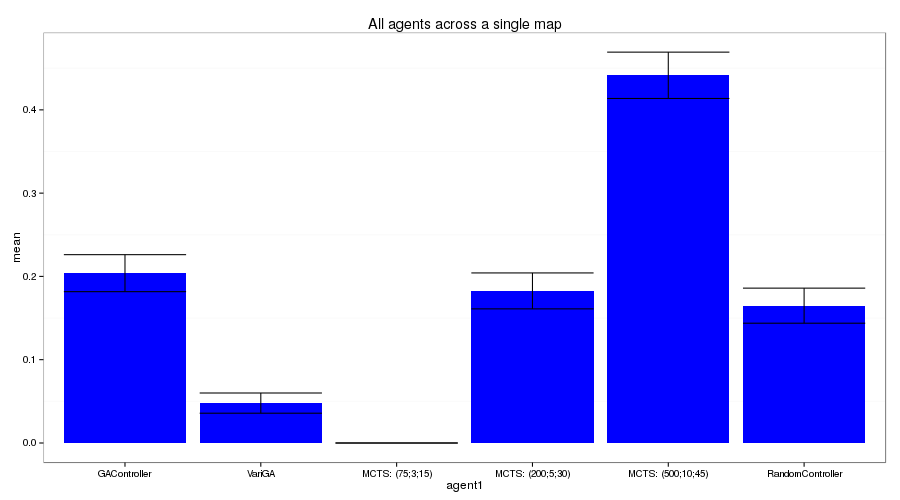
\includegraphics[width = \linewidth]{level5-txt-scores}
\caption{Average Score for each AI Agent over Map 5}
\label{avgScoreMap5}
\end{figure}

Level 5 - shown in Figure \ref{Level5State} - poses a particular problem for many of the agents (see Figure \ref{avgScoreMap5}). The asymmetric nature of the level, and the delayed reward caused great difficulty for the Agents. Relying on two button presses and the other agent to get through the open doors - in order - greatly reduced performance. The top agent, \emph{High MCTS}, only managed an average score of $0.44$ compared to its total average of just over $0.8$.

\section{Conclusions}
In this paper, we found that a strong MCTS player can solve simple cooperative problems without requiring communication between agents. We also found that a number of other \gls{ai} techniques experienced difficulty when the problem became cooperative. Further work is required in this area.

\subsection{Further Work}
There is scope for more work in a number of areas.

\subsubsection{Communication}
More work can be conducted in the writing of AI's to use communication in order to complete these challenges better amongst themselves. A framework for communication would be devised - with the requirement for fairly \gls{ggp} like restrictions in mind.

\subsubsection{Optimisations}
Future work should also include some work to ensure that the \gls{ai} Agents have their parameters set correctly. The \emph{High MCTS} performed well - showing the power of having the correct parameters compared to the \emph{Low MCTS}. The \emph{VariGA} has 7 parameters that we simply didn't have time to correctly optimise for this experiment.

\subsubsection{Problem Domain}
More work can also be done on experimenting with the problem domain itself. Expanding the object types to include different techniques such as pickup-able objects that can be placed on \emph{Buttons}, \emph{Buttons} that remain active for a period of time after vacating them as well as potentially \emph{Doors} that will open permanently if all it's \emph{Buttons} are activated. The scope here is fairly limitless.

\bibliographystyle{IEEEtran}
\bibliography{ceec}

\end{document}